\documentclass{scrartcl}

\usepackage{amssymb}
\usepackage{amsmath}
\usepackage{cancel}		%for strikethroughs
\usepackage{tikz}

%from Žižek - The Plague of Fantasies (2nd Ed.), p. 223
%cf. Lacan - Seminar 20: On Feminine Sexuality, the Limits of Love and Knowledge, p. 90

\begin{document}
	
	\hspace{3.5cm}
	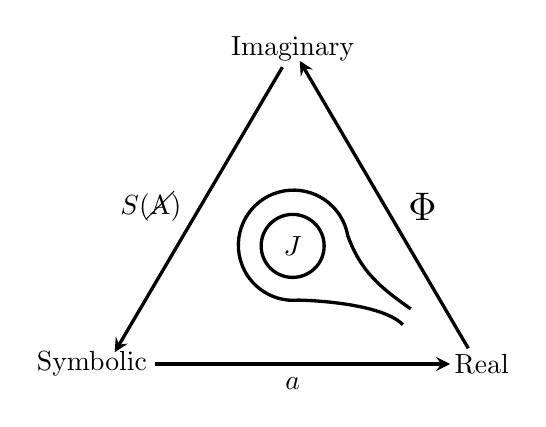
\begin{tikzpicture}[>=stealth]
	%lines
	%\draw[very thick] (0,0)--(-2.35,-4)--(2.35,-4)--(0,0);
	\draw[->,very thick] (-0.13,-0.23)--(-2.26,-3.85);
	\draw[->,very thick] (-1.75,-4)--(2,-4);
	\draw[->,very thick] (2.23,-3.8)--(0.09,-0.15);
	
	%labels
	\node at (0,-2.5)	{$J$};
	\node at (0,0)		{Imaginary};
	\node at (-2.55,-4)	{Symbolic};
	\node at (2.4,-4)	{Real};
	\node at (0,-4.25)	{$a$};
	\node at (1.65,-2)	{{\Large $\Phi$}};
	\node at (-1.8,-2)	{$S(\cancel{\text{A}})$};
	
	%circles
	\draw[very thick] (0,-2.5) circle (0.4cm);
	\draw[very thick] (0.7,-2.37) arc (10:275:0.7cm);
	\draw[very thick] (0.7,-2.37) to[out=290,in=145] (1.5,-3.3);
	\draw[very thick] (0.17,-3.19) to[out=180,in=135] (1.4,-3.5);
	
	%\draw[help lines] (-3,-5) grid (3,1);
	\end{tikzpicture}
	
	\vspace{0.75cm}
	
	{\small ``Let us first explain the schema itself. The three angles of the triangle stand for the three fundamental dimensions which, according to Lacan, structure the human universe: the Real (the `hard', traumatic reality which resists symbolization), the Symbolic (the field of language, of symbolic structure and communication), and the Imaginary (the domain of images with which we identify, and which capture our attention), $J$ in the middle of the triangle designates \textit{Jouissance}, the abyss of traumatic/excessive enjoyment which threatens to swallow us up, and towards which the subject desperately endeavours to maintain a proper distance (like the hero in Poe's `A Descent into the Maelstrom', who barely succeeds in not being dragged into the maelstrom). The three objects on the sides of the triangle specify the three ways in which to 'domesticate' or `normalize' this horrible Thing in the middle, to perceive it in a way which is no longer directly threatening: $S(\cancel{\text{A}})$ is the signifier of the barred Other (\textit{Autre}), and marks the inherent inconsistency of the symbolic order, the fact that there is something (\textit{jouissance}) which resists symbolization and causes gaps and ruptures in the symbolic order; $a$, the Lacanian \textit{objet petit a}, is the partial object which sets in motion the metonymic movement of desire (nose, feet, hair ... in perversion); the capital Phi is the fascinating image which represents the impossible Thing (the \textit{femme fatale} in the \textit{noir} universe, for example).}
	
	\vspace{0.15cm}
	
	{\small ``The matrix of these objects accounts for the three modes of depicting the sexual act: comicality, perversion, pathetic ecstasy. In the comic mode, the gap which separates the sexual act from our everyday social interaction is rendered palpable; in perversion, the focus is displaced on to a partial object which acts as a stand-in for the impossible-unrepresentable act itself (for Lacan, the ultimate example of such a partial object is \textit{the gaze itself}: what ultimately fascinates the pervert is the gaze transfixed by some traumatic Thing which can never be rendered present, like the stare of Medusa's head); finally, one can endeavour to erect a fascinating image destined to render present the pathos of the act.'' (\v{Z}i\v{z}ek, 1997: 222-3)}

\end{document}